%% ===================================================================
%%  CSE 402 -- presentation deck (beamer)
%%  BUILD:  pdflatex slides.tex   (twice)  or  build.bat
%% ===================================================================
\documentclass[aspectratio=169,11pt]{beamer}

\usepackage[T1]{fontenc}
\usepackage{lmodern}
\usepackage{booktabs}
\usepackage{graphicx}
\usepackage{amsmath}
\usepackage{tikz}
\usetikzlibrary{arrows.meta, positioning, shapes.geometric}

%% ---- a clean, quiet theme -----------------------------------------
\usetheme{default}
\usecolortheme{default}
\setbeamertemplate{navigation symbols}{}

\definecolor{ink}{HTML}{14161A}
\definecolor{deep}{HTML}{184F95}
\definecolor{blue}{HTML}{2A78D6}
\definecolor{red}{HTML}{E34948}
\definecolor{aqua}{HTML}{1BAF7A}
\definecolor{amber}{HTML}{EDA100}
\definecolor{violet}{HTML}{4A3AA7}
\definecolor{band}{HTML}{F2F5F9}
\definecolor{soft}{HTML}{4D5158}

\setbeamercolor{structure}{fg=deep}
\setbeamercolor{frametitle}{fg=white, bg=deep}
\setbeamercolor{normal text}{fg=ink}
\setbeamercolor{block title}{fg=white, bg=blue}
\setbeamercolor{block body}{bg=band}
\setbeamerfont{frametitle}{size=\large, series=\bfseries}
\setbeamerfont{framesubtitle}{size=\small}
\makeatletter
% Auto-height title bar: a fixed ht/dp clips any title that wraps to two lines.
\setbeamertemplate{frametitle}{%
  \nointerlineskip
  % `sep` pads on all sides AND grows the box, so a two-line title never clips
  \begin{beamercolorbox}[wd=\paperwidth,sep=0.9ex,leftskip=0.75em,
                         rightskip=0.75em]{frametitle}
    \usebeamerfont{frametitle}\insertframetitle%
    \ifx\insertframesubtitle\@empty\else
      {\ \ \usebeamerfont{framesubtitle}\normalfont\insertframesubtitle}%
    \fi
  \end{beamercolorbox}
}
\makeatother
\setbeamertemplate{itemize item}{\color{blue}\textbf{--}}
\setbeamertemplate{itemize subitem}{\color{soft}$\cdot$}
\setbeamertemplate{footline}{%
  \hfill\usebeamerfont{normal text}\color{soft}\scriptsize
  CSE 402 \textbullet\ Group 02, Section C \quad
  \insertframenumber/\inserttotalframenumber\hspace{1.2em}\vspace{0.6ex}}

\newcommand{\hl}[1]{\textcolor{deep}{\textbf{#1}}}
\newcommand{\good}[1]{\textcolor{aqua}{\textbf{#1}}}
\newcommand{\bad}[1]{\textcolor{red}{\textbf{#1}}}

%% ===================================================================
\title{\textbf{Simulating and Optimising\\Emergency-Department Patient Flow}}
\subtitle{Replicating Lv et al.\ (2026) --- and going four steps further}
\author{Sudip Kumar Saha \and Ahnaf Akib Tanim \and Md.\ Shahjalal Rumman \and
        Md.\ Dulal Hossain \and Md.\ Shoaib Hossain}
\institute{CSE 402 --- Numerical Analysis, Simulation and Modeling Sessional\\
           Group 02, Section C}
\date{}

\begin{document}

%% ---------- 1. TITLE ------------------------------------------------
{\setbeamertemplate{footline}{}
\begin{frame}[plain]
  \maketitle
  \vspace{-1.2em}
  \begin{center}\small\color{soft}
  Base paper: Lv, Liu, Yan \& Wang (2026), \emph{Healthcare} 14(1):99
  \end{center}
\end{frame}}

%% ---------- 2. BASE PAPER: THE SCENARIO -----------------------------
\begin{frame}{The base paper \textnormal{(1/3)}: the scenario}{A tertiary-hospital ED in China}
\begin{columns}[T,onlytextwidth]
\begin{column}{0.55\textwidth}
\vspace{0.1em}
{\footnotesize Only triage \textcolor{blue}{\textbf{Level III}} (urgent) and
\textcolor{amber}{\textbf{Level IV}} (non-urgent) patients are modelled ---
Levels I--II are critical and bypass the queue entirely.}
\vspace{0.4em}

{\scriptsize
\begin{tabular}{@{}ll@{}}
\toprule
\textbf{Arrivals} & non-homogeneous Poisson, weekly \\
                  & cycle --- 1.7 to 23 patients/h \\
\textbf{Triage mix} & 25\% Level III / 75\% Level IV \\
\textbf{Waiting targets} & $T_3 = 30$ min \quad $T_4 = 120$ min \\
\textbf{Initial consult} & 5--15 min (mean 9.1) \\
\textbf{Diagnostics} & 60\% of patients: lab, X-ray, \\
                     & CT, ultrasound (+ report delay) \\
\textbf{Follow-up consult} & 5--25 min (mean 12.8) \\
\textbf{Physicians} & 5 morning / 5 afternoon / 3 night \\
\textbf{One run} & 1 week $\approx$ 2,280 patients \\
\bottomrule
\end{tabular}}
\vspace{0.4em}

{\scriptsize\color{soft} These imply a system at \hl{87\% load} --- where every
extra point of utilisation costs minutes of waiting.}
\end{column}
\begin{column}{0.43\textwidth}
\vspace{-0.3em}
\begin{center}
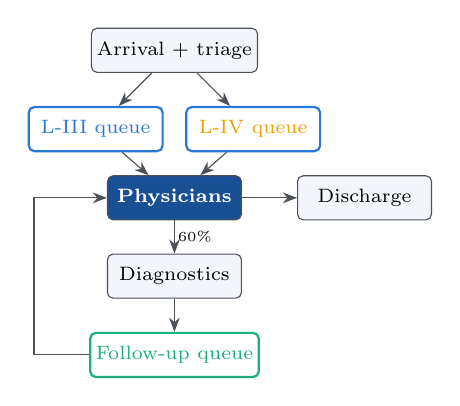
\begin{tikzpicture}[font=\scriptsize,
  node distance=4.2mm,
  box/.style={draw=soft, fill=band, rounded corners=2pt, minimum width=17mm,
              minimum height=5.6mm, align=center, inner sep=2pt},
  q/.style={box, fill=white, draw=blue, thick},
  a/.style={-{Stealth[length=1.8mm]}, draw=soft}]
\node[box] (arr) {Arrival + triage};
\node[q, below=of arr, xshift=-10mm] (q3) {\textcolor{blue}{L-III queue}};
\node[q, below=of arr, xshift=10mm] (q4) {\textcolor{amber}{L-IV queue}};
\node[box, fill=deep, text=white, below=8mm of arr, yshift=-5mm]
  (doc) {\textbf{Physicians}};
\node[box, right=7mm of doc] (out) {Discharge};
\node[box, below=of doc] (exam) {Diagnostics};
\node[q, below=of exam, draw=aqua] (qf) {\textcolor{aqua}{Follow-up queue}};
\draw[a] (arr) -- (q3);
\draw[a] (arr) -- (q4);
\draw[a] (q3) -- (doc);
\draw[a] (q4) -- (doc);
\draw[a] (doc) -- node[right,font=\tiny,inner sep=1pt]{60\%} (exam);
\draw[a] (doc) -- (out);
\draw[a] (exam) -- (qf);
\draw[a] (qf.west) -- ++(-7mm,0) |- (doc.west);
\end{tikzpicture}
\end{center}
\end{column}
\end{columns}
\end{frame}

%% ---------- 3. BASE PAPER: THE THREE POLICIES -----------------------
\begin{frame}{The base paper \textnormal{(2/3)}: three answers}{Lv et al.\ (2026), \emph{Healthcare} 14(1):99}
\vspace{-0.2em}
{\small A physician becomes free. \hl{Which of the three queues do they take
from?} The three policies differ only in how they answer that.}
\vspace{0.4em}

\begin{center}\footnotesize
\begin{tabular}{@{}p{2.3cm}p{5.0cm}p{4.6cm}@{}}
\toprule
\textbf{Policy} & \textbf{Rule} & \textbf{Consequence} \\
\midrule
\textcolor{red}{\textbf{IFP}}\newline Initial-First
  & New arrivals always first (L-III, then L-IV, then follow-ups)
  & Nobody breaches target, but follow-ups starve \\[0.3em]
\textcolor{amber}{\textbf{ALT}}\newline Alternating 1:1
  & At most half the doctors on new arrivals at once
  & L-III waits collapse; L-IV breaches \\[0.3em]
\textcolor{blue}{\textbf{SBP}}\newline Slack-Based
  & Urgent once waited $T_\ell - k_\ell$; two tunable dials $(k_1,k_2)$
  & Best of the three --- \emph{if} tuned well \\
\bottomrule
\end{tabular}
\end{center}
\vspace{0.5em}

\begin{block}{The slack idea, in one sentence}
\footnotesize $k_\ell$ is a \emph{head start}: with $T_3=30$ and $k_1=13.1$ a
Level III patient becomes ``urgent'' after $30-13.1 = 16.9$ min --- the system
starts rescuing them \hl{13.1 minutes before} they would breach. Bigger $k$ =
earlier rescue = more protection for that class, at everyone else's expense.
\end{block}
\end{frame}

%% ---------- 4. BASE PAPER: WHAT IT FOUND ----------------------------
\begin{frame}{The base paper \textnormal{(3/3)}: what it found}{100 replications per policy}
\vspace{-0.3em}
\begin{columns}[T,onlytextwidth]
\begin{column}{0.53\textwidth}
{\footnotesize\textbf{Reported performance}}
\vspace{0.25em}

{\footnotesize
\begin{tabular}{@{}lrrrr@{}}
\toprule
 & \textbf{Wait} & \textbf{L-III} & $\mathbf{SL_4}$ & \textbf{Util.} \\
\midrule
\textcolor{red}{IFP}   & 46.26 & 44.14 & 100\%  & 85.43\% \\
\textcolor{amber}{ALT} & 37.88 &  6.82 & 89.3\% & 85.41\% \\
\textcolor{blue}{SBP}  & \good{35.25} & 10.48 & 100\%  & 84.98\% \\
\bottomrule
\end{tabular}}
\vspace{0.45em}

{\footnotesize \hl{SBP wins}: $46.26 \rightarrow 35.25$ min, a
\good{$-23.8\%$} cut, with zero service-level violations.}
\vspace{0.5em}

{\footnotesize\textbf{How it tuned $(k_1,k_2)$}}
\vspace{0.2em}

{\scriptsize
\begin{tabular}{@{}lll@{}}
\toprule
\textbf{Stage} & \textbf{Step} & \textbf{Best} \\
\midrule
Coarse lattice & 1.0 & $(13,\,2)$ --- 36.38 min \\
Fine lattice   & 0.1 & $(13.1,\,2.1)$ --- 35.25 min \\
\bottomrule
\end{tabular}}
\vspace{0.45em}

{\scriptsize\color{soft} Validated with paired $t$-tests, Bonferroni
correction and Cohen's $d$ (all $>1.5$).}
\end{column}
\begin{column}{0.45\textwidth}
\vspace{-0.3em}
\begin{block}{Its other conclusions}
\scriptsize
\begin{itemize}\setlength\itemsep{0.12em}\setlength\parskip{0pt}
  \item Equipment runs at \hl{14--19\%}, physicians at \hl{85\%}
        $\Rightarrow$ \textbf{doctors are the bottleneck}
  \item More staff shortens waits, with diminishing returns
  \item The ranking survives a different service-time distribution
\end{itemize}
\end{block}

\begin{block}{What it does \emph{not} do}
\scriptsize
\begin{itemize}\setlength\itemsep{0.12em}\setlength\parskip{0pt}
  \item Optimise the \textbf{staffing level} --- it only probes it
  \item Compare against a \textbf{provably optimal} rule
  \item Use a real \textbf{numerical optimiser}
  \item Apply any \textbf{variance reduction}
  \item Release its engine or its dataset
\end{itemize}
\end{block}
\vspace{-0.2em}
{\scriptsize\color{soft}\centering Those five gaps are what we take on next.\par}
\end{column}
\end{columns}
\end{frame}

%% ---------- 5. WHAT WE DID ------------------------------------------
\begin{frame}{What we did}{Rebuild it from scratch, then push it four steps further}
\vspace{-0.3em}
\begin{center}\small
\begin{tabular}{@{}rp{5.4cm}p{6.0cm}@{}}
\toprule
& \textbf{What} & \textbf{Why it matters} \\
\midrule
\textbf{1} & \hl{Rebuild \& validate} the whole simulator from the published
             parameters alone
           & The paper releases neither code nor data --- we check every KPI
             it reports \\[0.35em]
\textbf{2} & Add a \hl{provably optimal} scheduling rule (the c$\mu$ rule)
           & The paper's three policies are all hand-designed heuristics \\[0.35em]
\textbf{3} & Replace brute-force search with a \hl{Nelder--Mead optimiser}
             under a real constraint
           & The lattice costs 50,415 simulations; we ask how few we need \\[0.35em]
\textbf{4} & Put a \hl{price} on waiting and salary, then optimise the
             \hl{staffing roster}
           & ``More doctors is better'' has no stopping point \\[0.35em]
\textbf{5} & \hl{Common random numbers} --- give every policy the identical
             simulated week
           & Sharpens every comparison without a single extra run \\
\bottomrule
\end{tabular}
\end{center}
\vspace{0.5em}
{\footnotesize\color{soft}
$\sim$7,900 lines of Python; hand-rolled \texttt{heapq} event loop (no SimPy);
33 automated correctness checks, all passing.}
\end{frame}

%% ---------- 5. VALIDATION -------------------------------------------
\begin{frame}{1. Does the rebuild match the paper?}{Structure yes, absolute level no}
\begin{columns}[T,onlytextwidth]
\begin{column}{0.47\textwidth}
\vspace{0.2em}
{\footnotesize
\begin{tabular}{@{}lrrr@{}}
\toprule
& \textbf{Ours} & \textbf{Paper} & \textbf{Dev.} \\
\midrule
\multicolumn{4}{@{}l}{\textbf{Reproduced closely}}\\
ALT L-III wait   & 6.05  & 6.82  & $-11\%$ \\
Utilisation      & 86.3\% & 85.4\% & $+1\%$ \\
Lab equipment    & 14.73\% & 14.36\% & $+0.4$pp \\
CT equipment     & 18.18\% & 17.64\% & $+0.5$pp \\
IFP service level& 100/100 & 100/100 & exact \\
\midrule
\multicolumn{4}{@{}l}{\textbf{Runs high}}\\
IFP mean wait    & 52.43 & 46.26 & $+13\%$ \\
SBP mean wait    & 44.08 & 35.25 & $+25\%$ \\
\bottomrule
\end{tabular}}
\vspace{0.7em}

{\scriptsize \textbf{Why?} The published parameters imply load
$\rho \approx 0.87$. Near saturation, waiting time is hypersensitive to the
last point of utilisation --- and the source dataset is not public.
\good{All 6 structural findings reproduce.}}
\end{column}
\begin{column}{0.51\textwidth}
\vspace{-0.6em}
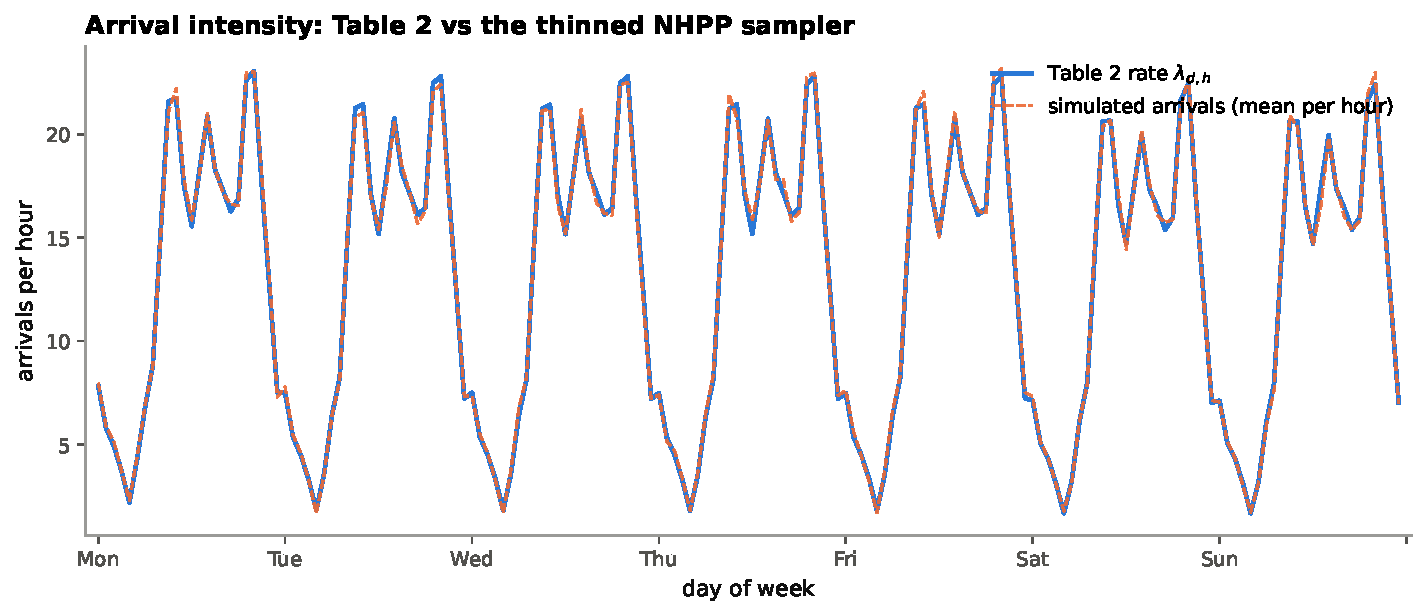
\includegraphics[width=\linewidth]{figures/wp1_arrival_validation.pdf}
\vspace{-0.4em}
{\scriptsize\color{soft} The arrival process, validated over 200 simulated
weeks: relative error \hl{1.67\%}, correlation \hl{0.9991}.}
\end{column}
\end{columns}
\end{frame}

%% ---------- 6. THE c-mu RULE ----------------------------------------
\begin{frame}{2. A rule with a proof behind it}{The c$\mu$ rule (Cox \& Smith, 1961)}
\begin{columns}[T,onlytextwidth]
\begin{column}{0.50\textwidth}
\vspace{0.3em}
{\small If class $\ell$ costs $c_\ell$ per minute of delay and takes
$1/\mu_\ell$ to serve, the \emph{cost-minimising} policy always serves the
class with the largest}
\[ \textcolor{deep}{\boxed{\,I_\ell = c_\ell \cdot \mu_\ell\,}} \]
{\small We set $c_\ell = 1/T_\ell$ --- a minute hurts in inverse proportion to
what that class tolerates.}
\vspace{0.5em}

{\footnotesize
\begin{tabular}{@{}lrrr@{}}
\toprule
\textbf{Class} & $T_\ell$ & $\mu_\ell$ & $\mathbf{c_\ell\mu_\ell}$ \\
\midrule
L-III initial & 30  & 0.110 & \textbf{0.003666} \\
Follow-up     & 60  & 0.078 & \textbf{0.001298} \\
L-IV initial  & 120 & 0.110 & \textbf{0.000916} \\
\bottomrule
\end{tabular}}
\vspace{0.5em}

{\scriptsize\color{soft} Indices are constants $\Rightarrow$ fixed priority.
We also implement the \emph{generalised} c$\mu$ rule,
$I_\ell = 2w\mu_\ell/T_\ell^2$, which adapts to how long the front patient has
waited --- and has \textbf{zero parameters to tune}.}
\end{column}
\begin{column}{0.48\textwidth}
\vspace{-0.5em}
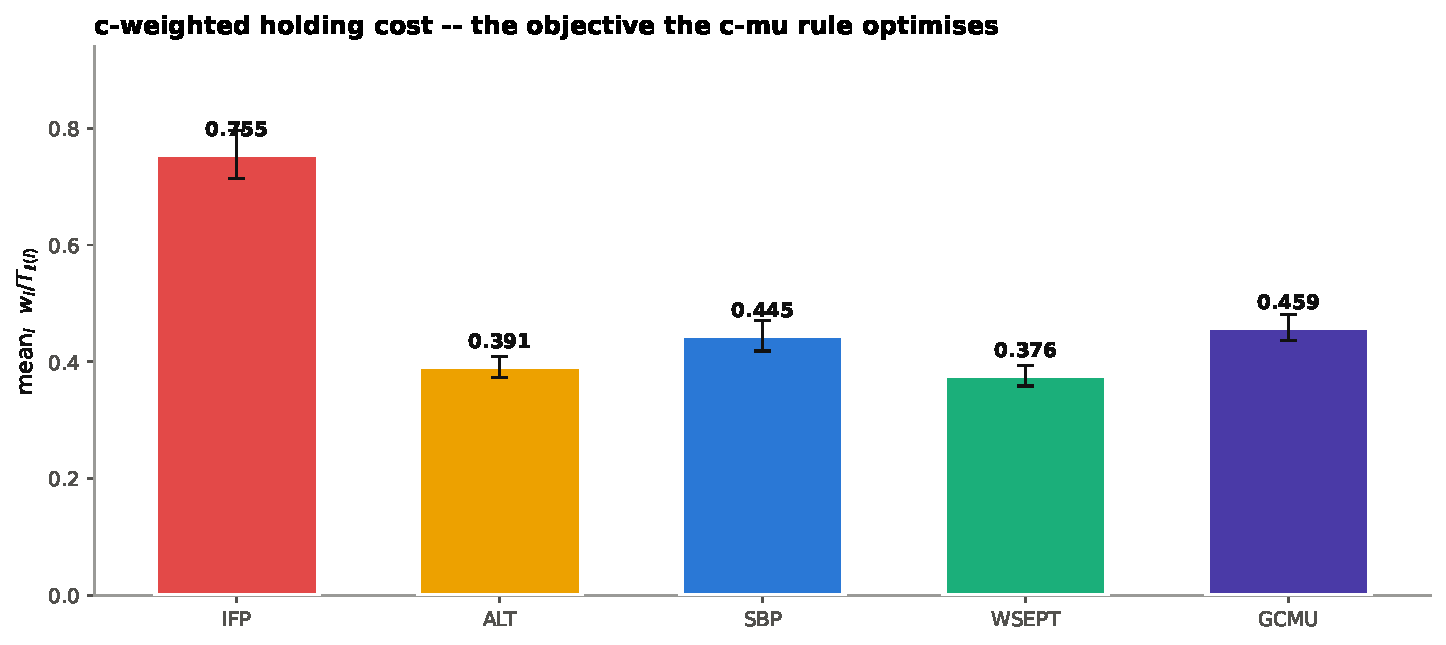
\includegraphics[width=\linewidth]{figures/wp2_holding_cost_bars.pdf}
\vspace{-0.3em}
{\scriptsize\color{soft} Judged on \emph{its own} objective --- waiting measured
in units of each patient's tolerance --- the c$\mu$ rule wins:
\good{0.376} vs IFP's \bad{0.755}, a 50\% reduction. On this system it also
gives the lowest raw mean wait (42.32 min).}
\end{column}
\end{columns}
\end{frame}

%% ---------- 7. THE OPTIMISER ----------------------------------------
\begin{frame}{3. A real optimiser instead of brute force}{Hand-implemented simplex + penalty function}
\begin{columns}[T,onlytextwidth]
\begin{column}{0.46\textwidth}
\vspace{0.1em}
{\footnotesize Minimise, subject to $SL_\ell \ge 95\%$:}
\vspace{-0.4em}
\[\textstyle\small F = \overline{W}
  + \mu \sum_\ell \max(0,\, SL^{\min}_\ell - SL_\ell)\]
\vspace{-1.1em}
{\footnotesize
\begin{itemize}\setlength\itemsep{0.15em}
  \item \hl{Same objective, same weeks} as the grid search
  \item Budget counted in \hl{simulations}, not seconds
  \item Noise handled by sample-average approximation
\end{itemize}}
\vspace{0.4em}

{\footnotesize
\begin{tabular}{@{}lrr@{}}
\toprule
\textbf{Method} & \textbf{Points} & \textbf{Sims} \\
\midrule
Grid search (paper's) & 2,332 & \bad{50,415} \\
Nelder--Mead          &    53 & \good{2,650} \\
\bottomrule
\end{tabular}}
\vspace{0.45em}

{\footnotesize\good{19$\times$ fewer simulations}; the two optima differ by
\hl{0.006 min}. Matches \texttt{scipy} to 0.0000.}
\end{column}
\begin{column}{0.52\textwidth}
\vspace{-0.6em}
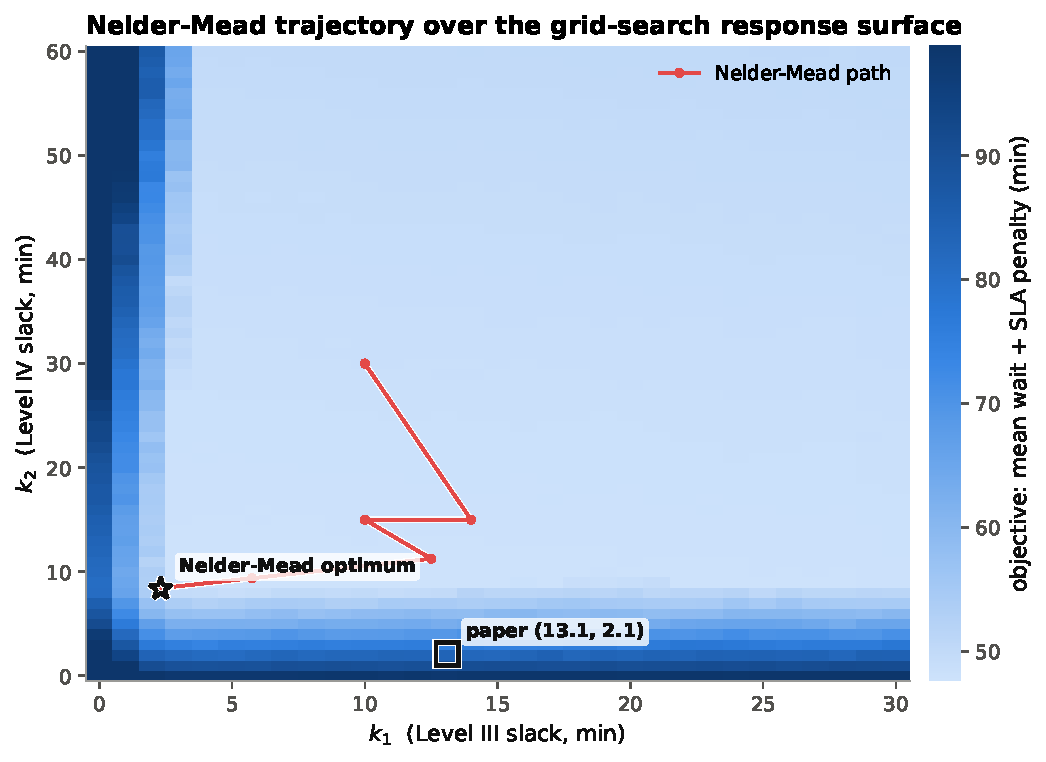
\includegraphics[width=\linewidth]{figures/wp3_simplex_path.pdf}
\vspace{-0.4em}
{\scriptsize\color{soft} The simplex walks down to the feasible optimum. The
dark band is the service-level penalty --- and \bad{the paper's own published
$(13.1, 2.1)$ sits inside it}: it reaches only 89.4\% on Level IV, because
$k_2=2.1$ rescues a patient at minute 117.9 of 120.}
\end{column}
\end{columns}
\end{frame}

%% ---------- 8. STAFFING ---------------------------------------------
\begin{frame}{4. How many doctors should the ED roster?}{Put a price on the trade-off}
\vspace{-0.2em}
\[\small
C(R,k_1,k_2) = \underbrace{\alpha\,H_{\text{phys}}}_{\text{salary}}
             + \underbrace{\beta\,W_{\text{total}}}_{\text{waiting}}
             + \underbrace{\gamma\,V_{\text{SLA}}}_{\text{breaches}}
\qquad R = (R_\text{morning},R_\text{afternoon},R_\text{night})
\]
\vspace{-0.6em}
\begin{columns}[T,onlytextwidth]
\begin{column}{0.53\textwidth}
{\footnotesize
\begin{tabular}{@{}llrrr@{}}
\toprule
& \textbf{Roster} & \textbf{Wait} & $SL_4$ & \textbf{Cost/wk} \\
\midrule
Paper & (5,5,3) & 44.18 & 95.6\% & 139,391 \\
$S_5$ & (6,7,5) & 4.32  & 100\%  & 124,082 \\
\textbf{Ours} & \textbf{(6,6,3)} & \textbf{10.97} & \textbf{99.9\%}
      & \good{110,513} \\
\bottomrule
\end{tabular}}
\vspace{0.6em}

{\small One more doctor on each \emph{day} shift, with thresholds re-tuned to
$(12.2,\,23.4)$: \good{$-20.7\%$ weekly cost}.}
\vspace{0.4em}

{\scriptsize\color{soft}\textbf{Why re-tune inside each roster?} The best
$(k_1,k_2)$ for a 3-doctor night is not the best for 5 --- $k_2$ moves from
8.4 to 23.4. Holding them fixed would score every alternative roster at
someone else's settings.}
\end{column}
\begin{column}{0.45\textwidth}
\vspace{0.1em}
{\footnotesize\textbf{Does the answer survive the assumptions?}}
\vspace{0.4em}

{\footnotesize
\begin{tabular}{@{}lll@{}}
\toprule
\textbf{Cost scenario} & \textbf{Winner} & \textbf{vs (5,5,3)} \\
\midrule
Baseline             & (6,6,3) & $-20.7\%$ \\
Waiting $\times 4$   & (6,7,3) & $-53.2\%$ \\
Waiting $\times$ 1/4 & (5,6,3) & $-5.2\%$ \\
Doctors $\times 1.5$ & (6,6,3) & $-12.4\%$ \\
Breach $\times 10$   & (6,6,3) & $-39.5\%$ \\
\bottomrule
\end{tabular}}
\vspace{0.7em}

{\scriptsize\color{soft} The winner \emph{moves} with the weights ---
\textbf{that is itself the finding.} The right staffing level depends on how a
hospital prices a waiting minute against a salary. But \good{every} weighting
beats the paper's (5,5,3).}
\end{column}
\end{columns}
\end{frame}

%% ---------- 9. CRN ---------------------------------------------------
\begin{frame}{5. Sharper statistics for free}{Common random numbers}
\vspace{-0.4em}
\begin{center}
$\operatorname{Var}(A-B) = \operatorname{Var}(A)+\operatorname{Var}(B)
 - 2\,\operatorname{Cov}(A,B)$
\quad\raisebox{0.15em}{\scriptsize\color{soft}
($\operatorname{Cov}=0$ with independent streams)}
\end{center}
\vspace{-0.3em}
\begin{columns}[T,onlytextwidth]
\begin{column}{0.36\textwidth}
\vspace{0.1em}
{\footnotesize
Give both policies the \hl{identical week} and a busy week inflates both
together: $\operatorname{Cov}\to1$, so the variance of the \emph{difference}
collapses.}
\vspace{0.5em}

{\footnotesize
\begin{tabular}{@{}lr@{}}
\toprule
Correlation induced & $+0.996$ \\
Variance removed & \good{98.95\%} \\
Efficiency gain & \good{95.8$\times$} \\
\bottomrule
\end{tabular}}
\vspace{0.5em}

{\scriptsize\color{soft} The whole patient stream is generated \emph{before}
the run, so patient \#1723 is bit-identical under every policy. Not a bias:
each policy's own mean and s.d.\ are unchanged.}
\end{column}
\begin{column}{0.62\textwidth}
\vspace{-0.5em}
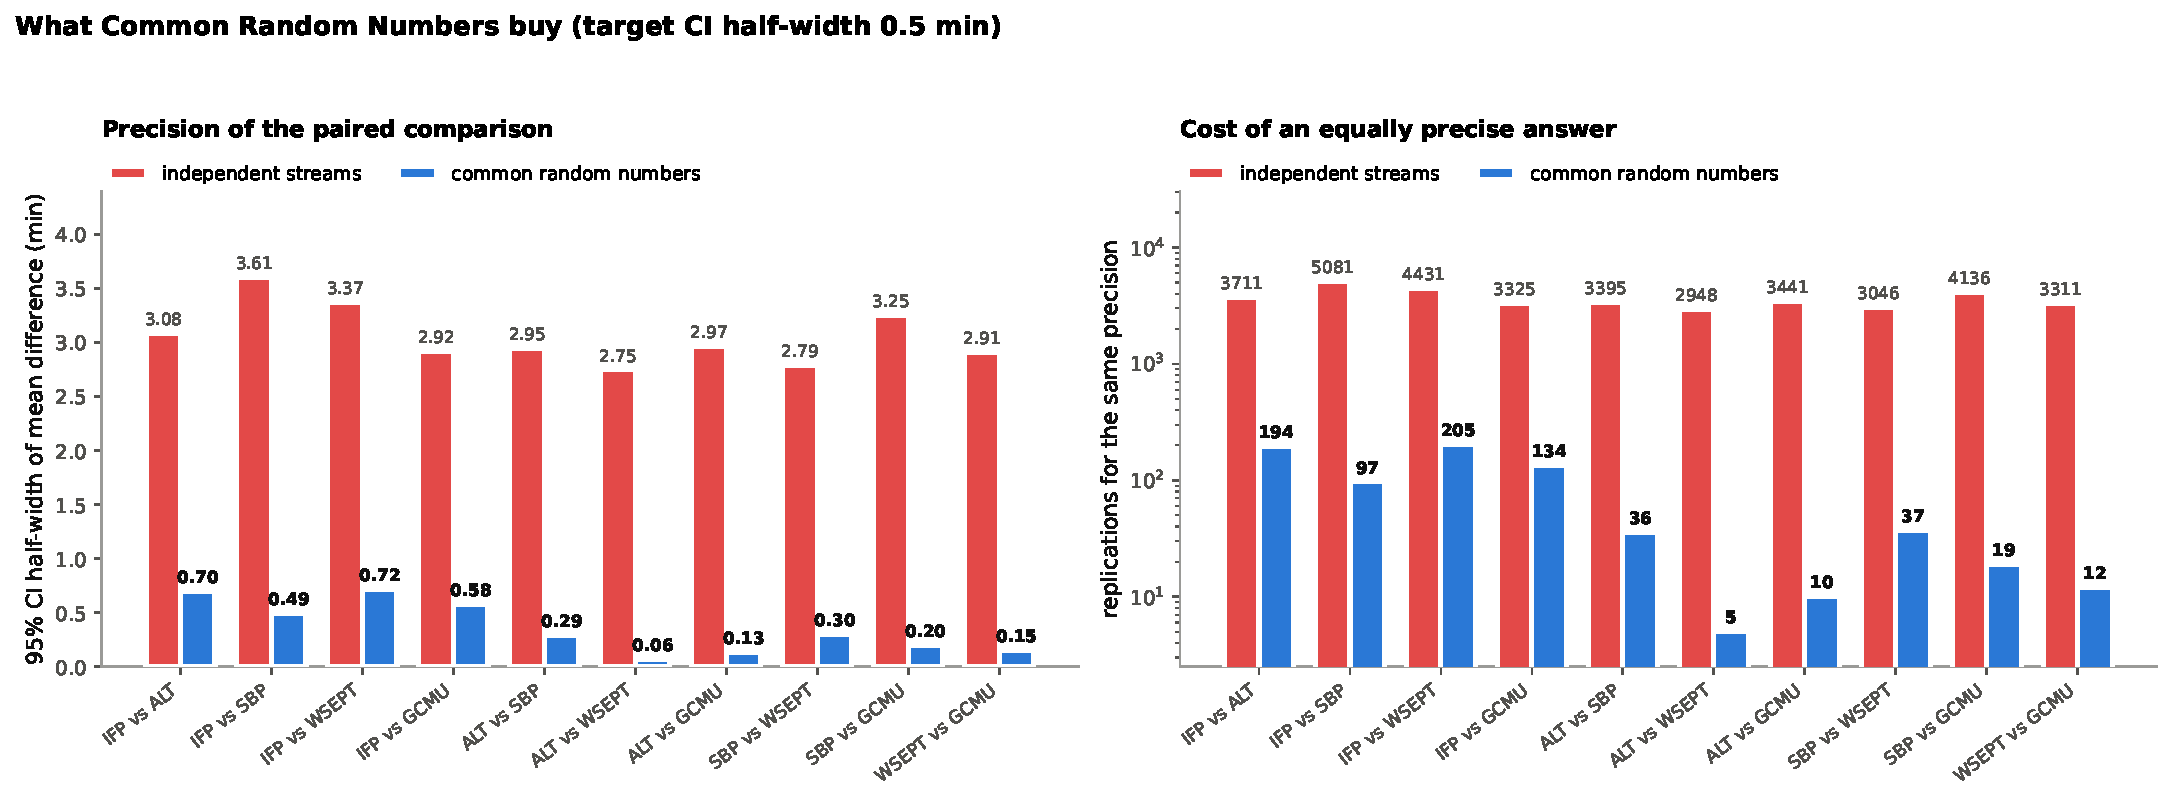
\includegraphics[width=\linewidth]{figures/wp5_crn_variance_reduction.pdf}
\vspace{-0.3em}
{\scriptsize\color{soft} Confidence intervals shrink 4--40$\times$;
replications needed for $\pm0.5$ min precision fall from thousands to dozens.
Practical reading: \textbf{20--30 CRN replications} beat the paper's 100
independent ones.}
\end{column}
\end{columns}
\end{frame}

%% ---------- 10. RESULTS WALKTHROUGH ---------------------------------
\begin{frame}{Results: all six policies, one table}{100 paired replications}
\vspace{-0.2em}
\begin{center}\footnotesize
\begin{tabular}{@{}llrrrrrc@{}}
\toprule
\textbf{Policy} & \textbf{Origin} & \textbf{Wait} & \textbf{L-III} &
\textbf{L-IV} & \textbf{Holding} & $\mathbf{SL_4}$ & \textbf{Meets SLA?} \\
\midrule
\textcolor{red}{IFP}    & base paper        & 52.43 & 50.88 & 52.94 & 0.7550 & 100.0\% & yes \\
\textcolor{amber}{ALT}  & base paper        & 42.39 &  6.05 & 54.61 & 0.3913 &  87.4\% & \bad{no} \\
\textcolor{blue}{SBP}   & base paper (13.1, 2.1) & 44.08 & 12.35 & 54.74 & 0.4450 & 89.4\% & \bad{no} \\
\textcolor{blue}{\textbf{SBP*}} & \textbf{ours} (2.31, 8.37) & 44.18 & 14.14 & 54.27 & 0.4570 & \good{95.6\%} & \good{yes} \\
\textcolor{aqua}{WSEPT} & \textbf{ours}, c$\mu$ & \good{42.32} & 3.76 & 55.30 & \good{0.3763} & 86.9\% & \bad{no} \\
\textcolor{violet}{Gc$\mu$} & \textbf{ours}, gen.\ c$\mu$ & 44.05 & 14.59 & 53.94 & 0.4588 & 91.0\% & \bad{no} \\
\bottomrule
\end{tabular}
\end{center}
\vspace{0.5em}

\begin{block}{There is no single winner --- and that is the result}
\small
\begin{tabular}{@{}p{4.1cm}p{3.7cm}p{4.9cm}@{}}
Shortest raw wait & \good{WSEPT} (42.32 min) & the c$\mu$ rule \\
Lowest holding cost & \good{WSEPT} (0.3763) & its own optimal objective \\
\textbf{Fastest that meets the SLA} & \good{SBP*} (44.18 min)
  & \textbf{the only adoptable one} \\
\end{tabular}
\end{block}
\vspace{0.2em}
{\scriptsize\color{soft} All 15 pairwise differences tested with paired
$t$-tests, Bonferroni-corrected ($\alpha_{\text{adj}}=0.00333$); 12 of 15
significant.}
\end{frame}

%% ---------- 11. TRADE-OFF + ROBUSTNESS ------------------------------
\begin{frame}{Comparative analysis: the whole study in two pictures}
\begin{columns}[T,onlytextwidth]
\begin{column}{0.49\textwidth}
\begin{center}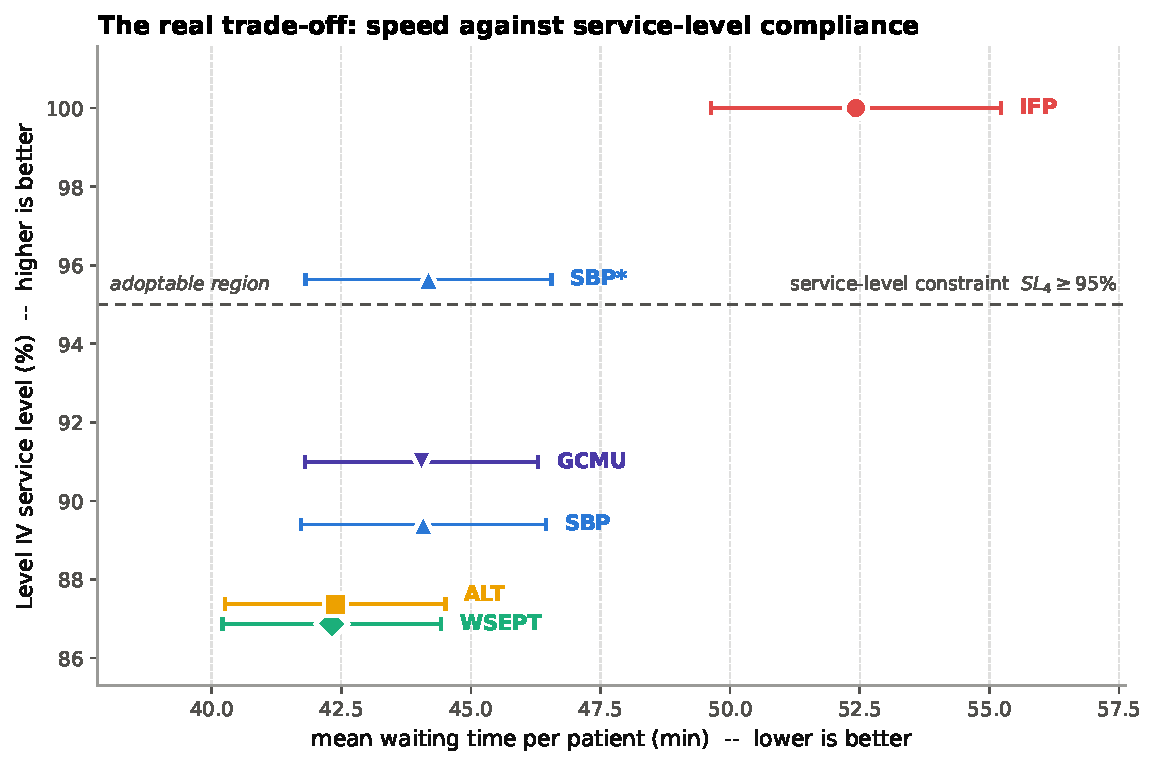
\includegraphics[width=\linewidth]{figures/final_tradeoff.pdf}\end{center}
\vspace{-0.5em}
{\scriptsize\color{soft}\textbf{Speed vs.\ compliance.} Only policies above the
dashed 95\% line are adoptable. IFP is safe but slow; the fast rules all
breach; \good{only SBP* is both}.}
\end{column}
\begin{column}{0.49\textwidth}
\begin{center}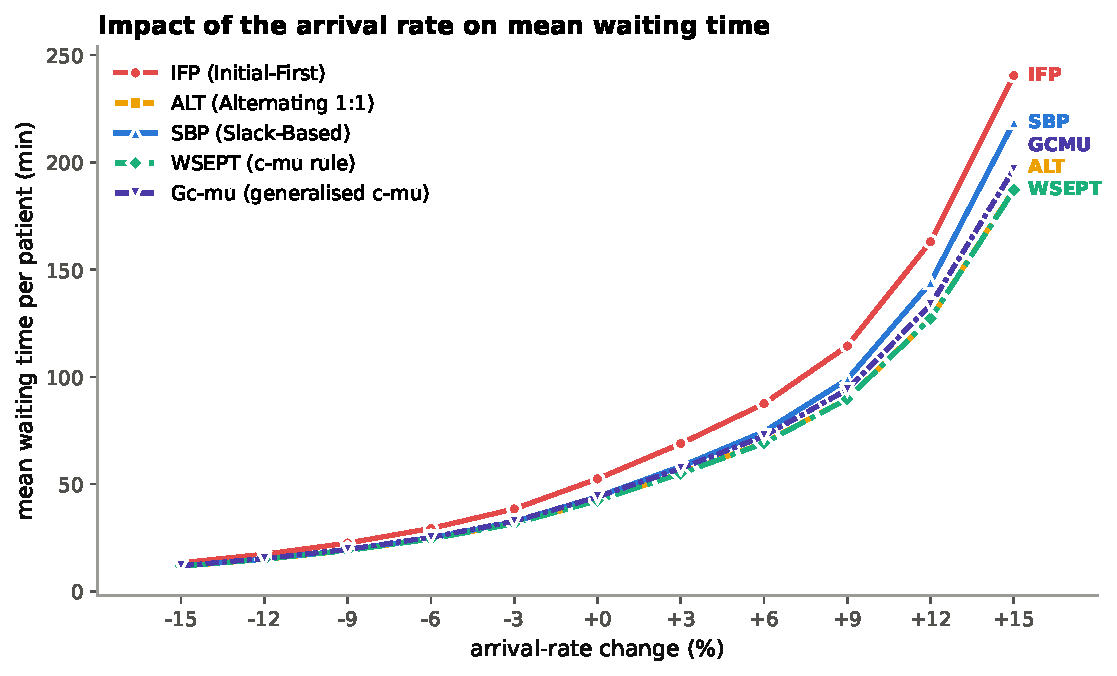
\includegraphics[width=\linewidth]{figures/sens_arrival_rate.pdf}\end{center}
\vspace{-0.5em}
{\scriptsize\color{soft}\textbf{Robustness.} Under light load the policies are
interchangeable; as the ED saturates the choice of rule is worth minutes per
patient. Reproduces the paper's Figure 4 --- as do its staffing and
lognormal-service-time checks.}
\end{column}
\end{columns}
\end{frame}

%% ---------- 12. CONCLUSION ------------------------------------------
\begin{frame}{Takeaways}
\vspace{-0.2em}
\begin{columns}[T,onlytextwidth]
\begin{column}{0.56\textwidth}
\begin{block}{What we established}
\small
\begin{itemize}\setlength\itemsep{0.35em}
  \item The paper's model \good{reproduces structurally} --- all 6 findings,
        equipment table within 0.5 pp
  \item A \good{provably optimal} rule beats all three heuristics on the
        delay-cost objective
  \item Nelder--Mead reaches the same optimum with \good{19$\times$ fewer}
        simulations
  \item The cost-optimal roster \good{(6,6,3)} saves \good{20.7\%} per week
  \item CRN removes \good{98.9\%} of comparison variance
\end{itemize}
\end{block}
\end{column}
\begin{column}{0.42\textwidth}
\begin{block}{The finding we did not expect}
\small On our model the paper's own published thresholds $(13.1,\,2.1)$
\bad{violate the 95\% Level IV constraint}.
\vspace{0.4em}

\hl{Published scheduling parameters are properties of the system they were
fitted to --- not transferable constants.}
\end{block}
\vspace{0.4em}
{\footnotesize\textbf{Next:} per-shift thresholds, a re-entrant c$\mu$ bound,
and a two-stage stochastic program for the roster.}
\end{column}
\end{columns}
\vspace{0.6em}
\begin{center}\small\color{soft}
Code, all result tables, figures and a full provenance log:
\texttt{github.com/Ahnaf-Akib-Tanim/Numeric-Project-submission}
\end{center}
\end{frame}

%% ---------- 13. THANK YOU ------------------------------------------
{\setbeamertemplate{footline}{}
\begin{frame}[plain]
\vfill
\begin{center}
{\Large\bfseries\color{deep} Thank you}\\[0.8em]
{\small Questions?}\\[1.6em]
{\footnotesize\color{soft}
Sudip Kumar Saha \textbullet\ Ahnaf Akib Tanim \textbullet\ Md.\ Shahjalal Rumman
\textbullet\ Md.\ Dulal Hossain \textbullet\ Md.\ Shoaib Hossain\\[0.3em]
CSE 402 --- Group 02, Section C}
\end{center}
\vfill
\end{frame}}

\end{document}
